%This Document was created in April 2011 by Brian Schiller at Western Washington University
%As the creator of this document, I make no claims to its copyright, and freely allow its duplication and distribution, as long as no profit is made.
%Please share this with anyone you like, and feel free to make changes or additions.
%Last Modified September 2, 2011 by Brian Schiller
\documentclass[11pt]{article} 

%begins paragraphs with an empty line instead of a tab.
\usepackage[parfill]{parskip}  

%smaller section titles
%\usepackage[compact,small]{titlesec}

%creates smaller margins
\usepackage{fullpage} 

%math commands and symbols
\usepackage{amsmath, amssymb}

%Theorem and proof environments
\usepackage{amsthm}
\newtheorem{lem}{Lemma}

%allows for comment blocks and verbatim sections
\usepackage{verbatim} 

%preserves tabs in verbatim sections. Good for including source code in documents.
\usepackage{moreverb}

%Include collumns
\usepackage{multicol}

%allows for \includegraphics
\usepackage{graphicx}

%clickable URLs, sections names
\usepackage[pdfborder={0 0 0}]{hyperref}

\title{A Rudimentary Introduction to \LaTeX}
\author{Brian Schiller}
\date{April 4, 2010}

\begin{document}
\maketitle
\tableofcontents

\newpage

\section{Introduction}
\LaTeX \,is different from WYSIWYG text editors such as Microsoft Word in that control structures are typed alongside the text. For example, rather than clicking a series of toolbar buttons to get center-justified text:
\begin{center}
	The center of the Earth is composed primarily of a nickel-iron alloy.
\end{center}
We instead type \begin{verbatimtab}
\begin{center} 
	The center of the Earth is composed primarily of a nickel-iron alloy.
\end{center}
\end{verbatimtab}
\LaTeX \,is also case-sensitive. In Math mode (which we will get to later), typing {\verb \delta } produces \(\delta\), but typing {\verb \Delta } produces \(\Delta\).

Required parameters of \LaTeX \,commands are placed inside curly braces \{ \ldots \}, and if there are any optional parameters, they are in square brackets [ \ldots ]. See the following section for some examples of this in the preamble.
	
\section{The Preamble}
The preamble is the area between {\verb \documentclass{...} } and {\verb \begin{document}. An example of a small preamble is
\begin{verbatimtab}
\documentclass[11pt]{article} 

%begins paragraphs with an empty line instead of a tab.
\usepackage[parfill]{parskip}  

%creates smaller margins
\usepackage{fullpage} 

%math commands and symbols
\usepackage{amsmath, amssymb}

% Theorem and proof environments
\usepackage{amsthm}

%allows for comment blocks and verbatim sections
\usepackage{verbatim} 

\title{A Rudimentary Introduction to \LaTeX}
\author{Brian Schiller}
\date{April 4, 2010}
\end{verbatimtab}

The preamble of a \LaTeX document is analogous to the declarations section of a program.
As well as \verb \usepackage  commands and title elements, there are a few other things you might want to include. The preamble is where you set choices that affect the entire document, such as page numbering, fonts, margins, and paper size.
%include subsections on particularly useful packages?
\section{Comments}
If you have done any programming you are probably familiar with comments. These are notes to yourself that won't show up in the laid-out document. For example, typing
\begin{verbatimtab}
\ldots all dogs have five legs: %check on this
three in front and two behind.
\end{verbatimtab}
will show up as 

\ldots all dogs have five legs: %check on this
three in front and two behind.

Comments are good way to blank out commands. Including the package `fullpage' changes the margins from the defaults (which are very big) to the more standard 1inch on each side. To switch between the two options, you can simply add or delete a \verb|%| before the command\\* {\verb \usepackage{fullpage} }. %notice that your editor probably thinks that "before the command..." is a comment. If you check the typeset document, you'll find that it is not. This is because of the {\verb % }, which is the inline version of the verbatim environment.

If you have a large section that you'd like to comment out, you can use a comment block. This requires loading the verbatim package, so make sure that you have {\verb \usepackage{verbatim} } in your preamble. The text
\begin{verbatimtab}
\begin{comment}
This paragraph is complete bogus. I don't want anyone to see it.

This one is junk as well.
\end{comment}
\end{verbatimtab}
does not typeset at all.

\section{Math Mode}
Math mode is different from text mode in a few subtle ways. 
\begin{samepage} %used to keep the list and the table on the same page.
\begin{description}
	\item[Spacing] in math mode squeezes everything very close together. Any spaces between parts of an equation are ignored. To force a space, you can use various commands, as seen in the table above. Note: units of em or ex are approximately the width of an M or X in a given font. These will scale with changes to font size. Other Note: These commands work in Text mode as well.
	\item[Empty Lines] are prohibited. You will get an error message when you try to typeset. If you want vertical space, you can use the command \verb|\vspace{...}|, with an argument in units of points, inches, centimeters, em or ex (eg: \verb|\vspace{0.5in}|).
	\item[Symbols] are treated differently. If you typeset \verb|2<5| in text mode you will get 2<5, but in math mode, you will get the expected \(2<5\).
\end{description}

	 \begin{table}[h] %adapted from http://crab.rutgers.edu/~karel/latex/class5/class5.html
	 \begin{center}
	 \begin{tabular}{ l l }
	 	%\hline
  		 \verb ||  &  \(||\) \\
	 	\verb |\,|  &  \(|\,|\) \\
	 	\verb |\;|  &  \(|\;|\) \\
	 	\verb |\quad|  &  \(|\quad |\) \\
	 	\verb |\qquad|  & \(|\qquad|\) \\
	 	\verb |\hspace{.5in}|  & \(|\hspace{.5in}|\) \\
	 	\verb |\hspace{5em}|  & \(|\hspace{5em}|\) \\
	 	\verb |\hspace{65pt}|  & \(|\hspace{65pt}|\) \\
	 \end{tabular}
      \caption{Horizontal Spacing in Math Mode}  %NOTE: this is within the center environment
	 \end{center}
	 \end{table} 
\end{samepage}	 
Math mode takes two different forms: Display and Inline. Inline math is used for small expressions that you want to typeset within a paragraph and is delimited by \verb \( on the left and \verb \) on the right. \verb \(x^2+y^2\leq4\) looks like this: \(x^2+y^2 \leq 4\). In Display mode, the same expression looks like
\[
x^2+y^2 \leq 4
\]
The difference is much more striking with large expressions such as
\begin{verbatimtab}
\int \limits_0^{v_{max}} v \,dv = \int \limits_0^a \frac{-g_0R^2}{(z+R)^2} \,dz
\end{verbatimtab}
which outputs \(\int \limits_0^{v_{max}} v\,dv = \int \limits_0^a \frac{-g_0R^2}{(z+R)^2} \,dz\) in inline mode, but in display mode looks like
\[
\int \limits_0^{v_{max}} v\,dv = \int \limits_0^a \frac{-g_0R^2}{(z+R)^2} \,dz
\]
\subsection{Subscripts and Superscripts}
Inside math mode, a superscript is produced by adding \verb|^{superscript}| to the object you want to have a superscript. Subscripts are the same, but \verb|^| is replaced by \verb|_|. The same construction is used for the limits of integrals and sums, as well as limits, as in the table. If your superscript or subscript is only one character, you can omit the curly braces.
\begin{table}
	\begin{center}
	\begin{tabular}{c | c}
	Input&Output \\
	\hline
	\verb|\lim_{a \to \infty} \, f(x) | & \(\displaystyle\lim_{a \to \infty} \, f(x)\)\\
	\verb|\int_0^4 \, f(x) \,\mathrm{d}x| & \(\displaystyle\int_0^4 \, f(x)\,\mathrm{d}x\)\\
	\verb|\sum_{n=1}^\infty \frac{1}{x^2}| & \(\displaystyle\sum_{n=1}^\infty \frac{1}{x^2}\) \\
	\end{tabular}
	\caption{Subscripts and Superscripts in Operators}
	\end{center}
\end{table}

\subsection{Fractions}
The fraction command has two arguments, one each for the top and bottom. It is typed as \verb|\frac{top}{bottom}|, and looks like \(\frac{top}{bottom}\) inline, compared with 
\[
\frac{top}{bottom}
\]
It is possible to force inline fractions to be larger by using \verb|\dfrac{top}{bottom}| instead of \verb|\frac|. The `d' stands for display. Compare \(\frac{1}{x^2+y^2}\) with \(\dfrac{1}{x^2+y^2}\). The display fraction will push lines of text apart, but is much easier to read. In general, if you want to have a display-size expression in the middle of a paragraph, you can prefix your command with \verb|\displaystyle|. Notice that \verb|\(\displaystyle\frac{1}{x^2+y^2}\)| produces \(\displaystyle\frac{1}{x^2+y^2}\), which looks the same as it did using \verb|\dfrac|. If the expression is more complicated the two will look different, as \verb|\displaystyle| applies to everything and \verb|\dfrac| applies only to that fraction.

\subsection{The Align Environment}
The align environment allows you to line up two or more formulas. Notice the equals signs in the following example, without the align environment on the left, with it on the right.
\begin{multicols}{2}
\[	v=\sqrt{\frac{mg}{\gamma}}\]
\[	35\ \frac{m}{s}=\sqrt{\frac{(0.025\ kg)(9.8\ \frac{m}{s^2})}{\gamma_0}} \]
\[	\gamma_0=\frac{(0.025\ kg)(9.8\ \frac{m}{s^2})}{35^2\ \frac{m^2}{s^2}}\]
\[	\gamma_0=0.0002 \ \frac{kg}{m}\]
\columnbreak
\begin{align*}
	v&=\sqrt{\frac{mg}{\gamma}}\\
	35\ \frac{m}{s}&=\sqrt{\frac{(0.025\ kg)(9.8\ \frac{m}{s^2})}{\gamma_0}} \\
	\gamma_0&=\frac{(0.025\ kg)(9.8\ \frac{m}{s^2})}{35^2\ \frac{m^2}{s^2}}\\
	\gamma_0&=0.0002 \ \frac{kg}{m}
\end{align*}
\end{multicols}
To use the align environment, type \verb|\begin{align*}| in place of \verb|\[| and \verb|\end{align*}| in place of \verb|\]|. Lines are separated using \verb|\\|. You should put an \verb|&| at the point of alignment. To produce the lines above right, type
\begin{verbatimtab}
\begin{align*}
	v&=\sqrt{\frac{mg}{\gamma}}\\
	35\ \frac{m}{s}&=\sqrt{\frac{(0.025\ kg)(9.8\ \frac{m}{s^2})}{\gamma_0}} \\
	\gamma_0&=\frac{(0.025\ kg)(9.8\ \frac{m}{s^2})}{35^2\ \frac{m^2}{s^2}}\\
	\gamma_0&=0.0002 \ \frac{kg}{m}
\end{align*}
\end{verbatimtab}
The asterisk is there to prevent an equation label, which we don't go into here.%or do we? new section?%
Try leaving it out and see how it changes.

The align environment can also create two columns of aligned expressions. See this example from Math Into \LaTeX.
\begin{align*}
	x&=x \wedge (y \vee z) &&\text{(by distributivity)} \\
	&= (x \wedge y) \vee (x \wedge z) && \text{(by condition (M))}\\
	&= y \vee z.
\end{align*}
This is typeset as 
\begin{verbatimtab}
	\begin{align*}
		x&=x \wedge (y \vee z) &&\text{(by distributivity)} \\
		&= (x \wedge y) \vee (x \wedge z) && \text{(by condition (M))}\\
		&= y \vee z.
	\end{align*}
\end{verbatimtab}

\subsection{Matrices}
Matrices work in much the same way as aligned equations. Using an \verb|&| between elements, and a \verb|\\| after each line, type
\begin{verbatimtab}
\[ \begin{matrix}
	1&-3&3&-2 \\
	-3&7&-1&2\\
	0&1&-4&3\\ 
\end{matrix}\]
\end{verbatimtab}
to get 
\[ \begin{matrix}
	1&-3&3&-2 \\
	-3&7&-1&2\\
	0&1&-4&3\\ 
\end{matrix}\]
Notice that there are no bars on this matrix. You probably want some bars on that thing. Replace \verb|matrix| in the argument of \verb|\begin| with \verb|bmatrix|, \verb|pmatrix|,  \verb|vmatrix|, or \verb|Vmatrix| (notice the capital `V'). These produce, respectively, square brackets, parentheses, vertical bars, and double vertical bars. There is also a \verb|\begin{smallmatrix}| environment for matrices inside paragraphs.

\subsection{Theorems}
Each theorem-like environment that you will use needs to be declared in the preamble. For example, to have an environment called `Lemma,' you would need to first load the package \verb|amsthm|, and also include the line \verb|\newtheorem{lem}{Lemma}| The first argument, \verb|lem|, is a handle for the environment. The second argument is the title that will be displayed. 

You could now start a lemma in your document with \verb|\begin{lem}|.
\begin{lem}
If $p$ is prime and $p \mid ab$ then $p \mid a$ or $p \mid b$.
\end{lem}
Theorem-like environments (Lemmas, Theorems, Definitions, etc) are numbered automatically, but it is possible to change the numbering conventions or remove the numbers altogether. To remove them, replace the line in your preamble with \verb|\newtheorem*{lem}{Lemma}|. If you want to change the way theorems are numbered, you will have to do more research.

Proofs are comparatively very easy. Just type \verb|\begin{proof}|, then your proof, then \verb|\end{proof}|. Neither the proof nor theorem environment will enter Math Mode automatically.

\section{Tables}
Tables can be created using the \verb|tabular| environment, which takes one argument. The argument is the number and text-justification of the columns. `c' indicates center-justified, `l' is left-justfied, and `r' is right-justified. So, a table with three center-justified columns followed by two right-justified columns would start of like this: \verb|\begin{tabular}{c c c r r}|. Additionally, to include bars separating columns, put a `\textbar' (found above the enter key) between the c's l's and r's.

The contents of the table is formatted much like matrices, with an \& separating each cell in a given row. Rows are separated by two backslashes, \verb|\\|. If you would like a line between two rows, include the line \verb|\hline| between them.

You will often want a title or subtitle to a table which spans multiple columns. This is achieved with the \verb|multicolumn| command, which takes three arguments: The number of columns to span, the justification of the cell (c, l, or r), and the contents of the cell. A title spanning four columns, center-justified, with text `My Title' is entered as \verb|\multicolumn{4}{c}{My Title}|. The second argument can also contain a `\textbar' or two. The following is a table, along with the code to generate it:

\begin{multicols}{2}
\begin{center}
\begin{tabular}{c | c | c | c}
	Var & \multicolumn{3}{c}{Functions}\\
	$x$ & $2x$ & $x^2$ & $2x^2$ \\
	\hline
	-2 & -4 & 4 & 8\\
	-1 & -2 & 1 & 2\\
	0  & 0 & 0 & 0\\
	1 & 2 & 1 & 2\\
	2 & 4 & 4 & 8\\
\end{tabular}
\end{center}
\columnbreak

\begin{verbatimtab}
\begin{tabular}{c | c | c | c}
	Var & \multicolumn{3}{c}{Functions}\\
	$x$ & $2x$ & $x^2$ & $2x^2$ \\
	\hline
	-2 & -4 & 4 & 8\\
	-1 & -2 & 1 & 2\\
	0  & 0 & 0 & 0\\
	1 & 2 & 1 & 2\\
	2 & 4 & 4 & 8\\
\end{tabular}
\end{verbatimtab}
\end{multicols}



\section{Pictures}
Pictures are a complicated topic in \LaTeX. To some extent, they are a bit beyond the scope of this introduction. However, in the simplest case, makes sure that you've loaded the package \verb|graphicx|, and that the picture you want to include is in the same folder as your .tex file. \verb|\includegraphics{image.jpg}|, or whatever the picture is called. Here is a picture of a pair of boots.
\begin{center}
	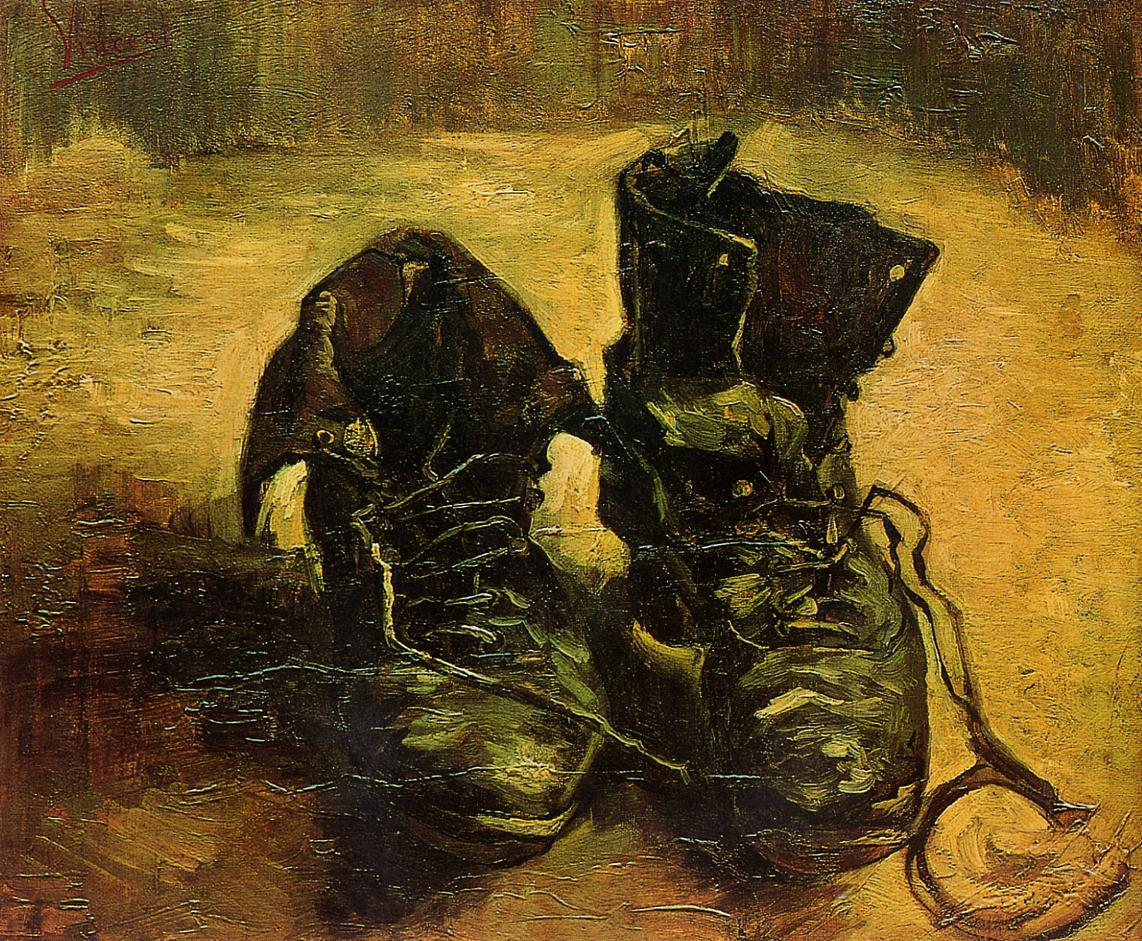
\includegraphics[keepaspectratio=true, width=0.5\textwidth]{vangogh_shoes.jpg}\\
	This painting was done by Vincent Van Gogh.\\
\end{center}

If you are compiling to a pdf, you can include image formatted as jpg, png, pdf, vector graphics, or eps (if you include the epstopdf package). However, if you compile to dvi format, only eps images can be included.

Pictures are scaled according to a number of optional parameters. The boots were produced with the following options.
\begin{verbatimtab}
\begin{center}
	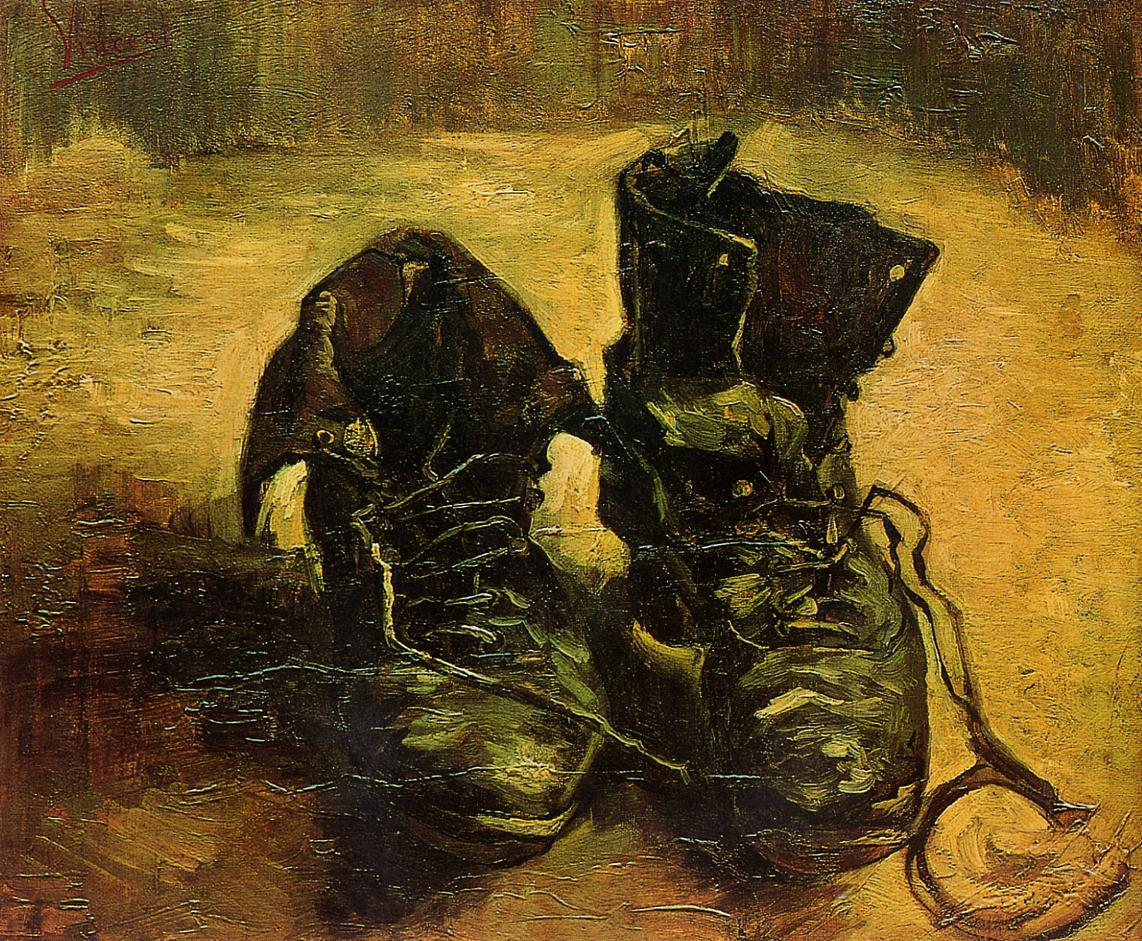
\includegraphics[keepaspectratio=true, width=0.5\textwidth]{vangogh_shoes.jpg}
\end{center}
\end{verbatimtab}

\section{Packages}
It's not a great idea to have a list of packages that you put at the start of every document you type, because there are sometimes conflicting declarations. If two packages each declare a command \verb|\start|, for example, \LaTeX{} will use the definition in the one declared last. That said, these are some packages I use often enough to mention. All of these packages are well-documented online.

\begin{description}
	\item[\hspace{4em} amsmath] This one almost goes without saying. 
	\item[\hspace{4em} verbatim] Permits comment blocks, as well as printing text exactly as you type it (\verb|even if it has control characters like $ and %|).
	\item[\hspace{4em} hyperref] Produces clickable URLs.
	\item[\hspace{4em} multicol] Allows you to have multiple columns.
	\item[\hspace{4em} geometry] Easy-to-use margin control and other layout details.
	\item[\hspace{4em} graphicx] Lets you include pictures in your documents.
	\item[\hspace{4em} listings] Very comprehensive package for including source code.
\end{description}

\section{Other Things}
Quotation marks in \LaTeX \,are tricky things. Using the usual key, \verb|"| from shift+apostrophe will look like "this," which is not necessarily desirable. instead, use \verb|`| or \verb|``| (found under the esc key) to open a quote, and apostrophe to close (\verb|'| or \verb|''|). This will look like ``this.''

There are several case-sensitive commands to change text size. The text to be changed should be inside a declare block (within a set of curly braces) with the command at the beginning. Type \verb|{\footnotesize speak softly and carry a big stick}|, to produce {\footnotesize speak softly and carry a big stick}. See the table for comparisons of text sizes.

\begin{table} [h!]
\begin{center}
\begin{tabular}{ l l | l l}
\textbf{Command}    &  \textbf{Typeset} & \textbf{Command}    &  \textbf{Typeset}\\ \hline
\verb=\tiny=      &  {\tiny sunflower}   & \verb=\textnormal{...}=            &  {\textnormal normal}        \\
\verb=\scriptsize=       &  {\scriptsize sunflower}  & \verb=\emph{...}=       &  \emph{emphasis}  \\
\verb=\footnotesize=    &  {\footnotesize sunflower} & \verb=\textsf{...}=           &  \textsf{sans serif}       \\
\verb=\small=           &  {\small sunflower}   & \verb=\texttt{...}=      &  \texttt{fixed width}  \\
\verb=\normalsize=      &  {\normalsize sunflower}  & \verb=\textit{...}=           &  \textit{italics}       \\
\verb=\large=           &  {\large sunflower}       & \verb=\textsc{...}=           &  \textsc{smallcaps}       \\
\verb=\Large=           &  {\Large sunflower}     & \verb=\uppercase{...}=        &  \uppercase{uppercase}       \\
\verb=\LARGE=        	&  {\LARGE sunflower}   & \verb=\textbf{...}=        	&  \textbf{bold font}        \\
\verb=\huge=        	&  {\huge sunflower}        \\
\verb=\Huge=        	&  {\Huge sunflower}        \\ \hline
\end{tabular}
     \caption{Font Sizes and Styles}
\end{center}
\end{table}
 \newpage

\section{Further Reading}
\begin{itemize}
	\item[--] These are good places to start if you're still working on installing \LaTeX. \\* \url{http://www.latex-project.org/ftp.html} \\* \url{http://latex101.wikispaces.com/TeX+clients}
	\item[--] If you just want a small equation typeset, this website will produce images and codes for email.  \url{http://www.texify.com/}
	\item[--] To look up a symbol, you can draw it and find matches. There are also iPhone and android versions. \url{http://detexify.kirelabs.org/classify.html}
	\item[--] This is a good general reference. \\* \url{http://tobi.oetiker.ch/lshort/lshort.pdf}
	\item[--] This is a very valuable reference to keep on hand if you're typing mathematical documents. It has the \TeX commands for lots of symbols, which largely assume the use of the amssymb package.\\* \url{http://tex.loria.fr/general/downes-short-math-guide.pdf}
	\item[--] This is where I first started learning \LaTeX. The whole book is not available here; the pages skip abruptly from 56 to 345, but its still quite a bit of information. We have a complete copy in the Math Center available for checkout. \\* \url{http://mirror.hmc.edu/ctan/info/mil/mil.pdf}.
	\item[--] \url{http://en.wikibooks.org/wiki/Latex}
	\item[--] There's lots of documentation available for \LaTeX \,online. The first place I look is usually \url{http://www.google.com/}.
\end{itemize}
\end{document}  